% ── Figure CUDA: thread → output-element mapping ─────────────
% Y_{J×K} shown as a 2×2 grid of 4×3-thread blocks (representative;
% actual blocks are 32×32). One highlighted thread does a serial
% dot product over the contracted index i.
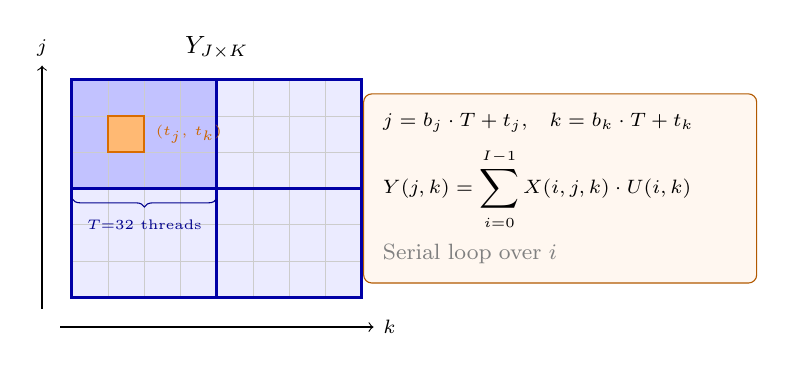
\begin{tikzpicture}[font=\small]

  % cell size (visual units, not physical scale)
  \def\cs{0.46}

  %────────────────────────────────────────────────────────────
  % Output matrix Y  (8 cols = j-axis, 6 rows = k-axis)
  %────────────────────────────────────────────────────────────

  % base cells
  \foreach \j in {0,...,7} {
    \foreach \k in {0,...,5} {
      \fill[blue!8] ({0.46*\j}, {0.46*\k})
        rectangle ({0.46*\j+0.46}, {0.46*\k+0.46});
      \draw[gray!40, line width=0.2pt] ({0.46*\j}, {0.46*\k})
        rectangle ({0.46*\j+0.46}, {0.46*\k+0.46});
    }
  }

  % highlight block (bj=0, bk=1): j∈[0,3], k∈[3,5]
  \foreach \j in {0,...,3} {
    \foreach \k in {3,...,5} {
      \fill[blue!24] ({0.46*\j}, {0.46*\k})
        rectangle ({0.46*\j+0.46}, {0.46*\k+0.46});
      \draw[gray!40, line width=0.2pt] ({0.46*\j}, {0.46*\k})
        rectangle ({0.46*\j+0.46}, {0.46*\k+0.46});
    }
  }

  % block outlines (2×2 grid of 4×3-thread blocks)
  % bj=0,bk=0
  \draw[blue!65!black, line width=1.1pt] (0,    0   ) rectangle (1.84, 1.38);
  % bj=1,bk=0
  \draw[blue!65!black, line width=1.1pt] (1.84, 0   ) rectangle (3.68, 1.38);
  % bj=0,bk=1  (highlighted block)
  \draw[blue!65!black, line width=1.1pt] (0,    1.38) rectangle (1.84, 2.76);
  % bj=1,bk=1
  \draw[blue!65!black, line width=1.1pt] (1.84, 1.38) rectangle (3.68, 2.76);

  % highlighted thread: j=1, k=4  →  x∈[0.46, 0.92], y∈[1.84, 2.30]
  \fill[orange!55] (0.46, 1.84) rectangle (0.92, 2.30);
  \draw[orange!85!black, line width=0.75pt] (0.46, 1.84) rectangle (0.92, 2.30);

  % matrix label
  \node[above, font=\small\bfseries] at (1.84, 2.90) {$Y_{J\times K}$};

  % axes
  \draw[->, thin] (-0.15, -0.38) -- (3.83, -0.38)
    node[right, font=\scriptsize] {$k$};
  \draw[->, thin] (-0.38, -0.15) -- (-0.38, 2.94)
    node[above, font=\scriptsize] {$j$};


  % brace: T threads per block dimension
  \draw[decorate, decoration={brace, amplitude=3pt, mirror},
        blue!55!black, thin]
    (0, 1.38-0.13) -- (1.84, 1.38-0.13)
    node[midway, below=4pt, font=\tiny, blue!55!black] {$T{=}32$ threads};

  % thread label beside highlighted cell
  \node[orange!80!black, font=\tiny, right] at (0.94, 2.07)
    {$(t_j,\,t_k)$};


  %────────────────────────────────────────────────────────────
  % Per-thread computation box
  %────────────────────────────────────────────────────────────
  \node[draw=orange!70!black, rounded corners=3pt, fill=orange!6,
        text width=4.5cm, align=left, font=\scriptsize,
        inner sep=7pt] at (6.2, 1.38)
  {
    $j = b_j \cdot T + t_j$,\quad $k = b_k \cdot T + t_k$ \\[5pt]
    $\displaystyle Y(j,k) = \sum_{i=0}^{I-1} X(i,j,k) \cdot U(i,k)$ \\[4pt]
    \textcolor{gray}{\footnotesize Serial loop over $i$}
  };

\end{tikzpicture}
